\section*{a) Understanding the problem}

The problem stated in the project is very similar to the problem of finding a minimum spanning tree (MST) in a graph, with an important difference. Here, each edge is paired with another edge in the graph, possibly itself. If the edges are $E=\{e_1,e_2,\dotsc,e_m\}$, then edge $e_i$ is paired with edge $e_{m+1-i}$ and these edges are called each others' 'mirror'. 

In colloquial terms, the problem is to determine if there exists a spanning tree $T$ in the graph $G$ with a mirror $M$ such that the weight of $T$ and $M$ are both below the threshold $B$. The weight of a spanning tree is defined as the sum of the weights of its edges, and its mirror $M$ is defined as the set of edges that are the mirror edges of the edges in $T$. The weight of a set of edges is denoted $|\cdot|$.

Importantly, while there is a restriction that the edges in $T$, namely that they form a spanning tree of $G$, there is no restriction on the edges in $M$. These can belong to $T$ or some other part of $G$ and generally be thought of as a random subset of $(n-1)$ edges. 

This problem is computationally hard to solve, as this report will show. As an example, the solution to the first example problem is shown below. 

\begin{figure}[h]
    \centering
    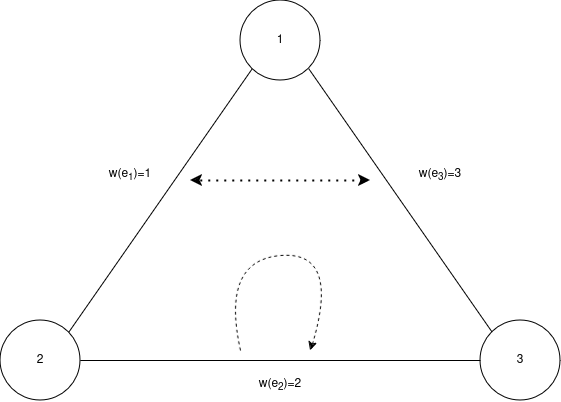
\includegraphics[width=0.7\linewidth]{Latex/Billeder/a_example.png}
    \caption{First example, where the dotted lines illustrate an edge's mirror edge.}
    \label{fig:a_example}
\end{figure}

For $B=4$, the answer is "YES". This is because the edges $T=\{e_1,e_3\}$ with mirror $M=\{e_3,e_1\}$ have the weights $|T|=|M|=4\leq B$.  
